\documentclass[11pt]{amsbook}

%\usepackage{../HBSuerDemir} 


\usepackage{amsmath}
\usepackage{graphicx}



\begin{document}

%\hPage{b1p2/320}

circle (or a center) and gradually receding from or approaching \\
it.\\ Two examples of spiral are \\ 

$1) r=a^\theta \quad (ARCHİMEDES' Spiral)\\$
$2) a^\theta =\ln r \quad or \quad r=e^{a\theta } \quad (logarithmic \quad Spiral )(See\quad Chapter \quad6.)\\$


\quad1. An ARCHIMEDES' Spiral is the trajectory of a point P . .
moving uniformly on a line which in turn rotating uniformly about
about a point. 


\indent Taking the center 0 of rotation\\
as pole and thet line when P is at 0\\
as polar axis, we have
\begin{figure}[h]

\hspace*{6cm}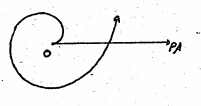
\includegraphics{images/image1.jpg}

\end{figure}
$$r=bt(linear motion on 0r)$$
$$\theta=wt(uniform rotation)$$
$$r=bt=b.\frac{\theta}{\omega}=\frac{b}{\omega}\theta=a\theta$$
\indent If $ a>0 $, having $r \rightarrow \infty $ as $ \theta \rightarrow \infty $, the curve is a spiral\\
admitting CPA as axis of symmetry(since $r \rightarrow -r$ when $\theta \rightarrow - \theta$ ),\\
with PA as tangent at 0. (when $a<0$, the motion takes place\\
in clockwise sense ).\\
\indent In the history of mathematics this curve is the first\\
curve other than the circle to which tangent line has been cons-\\
tructed. Also Archimedes used this curve to tricest an angle and\\
squaring a circle.\\
\indent 2. The curve $r=e^{a\theta} \quad (a>0)$ is another \\
spiral since $r \rightarrow $ as $\theta \rightarrow \infty$. Furthermore since \\
$r \rightarrow 0$ as $\theta \rightarrow -\infty $, he pole is a point-asymptote.
\begin{figure}[h]

\hspace*{6cm}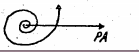
\includegraphics{images/image2.png}\\
\indent Among other spirals we mention the following.\\
\indent 3. $r\theta=a$ (hyperbolic or reciprocal spiral)

\end{figure}






\end{document}
